\documentclass{article} 

\usepackage[margin=0.9in]{geometry}
%\usepackage{subfig}
\usepackage{amsmath}
\usepackage{amsfonts}
\usepackage{amssymb}
\usepackage{amsthm}
\usepackage{graphicx}
\usepackage[hidelinks]{hyperref}
% \usepackage{showlabels}
\usepackage{lineno}
% \linenumbers
\usepackage{natbib}

\newtheorem{lemma}{Lemma}
\newtheorem{prop}{Proposition}
\newtheorem{thm}{Theorem}
\newtheorem{prob}{Problem}
\newtheorem{defn}{Definition}
\newtheorem{obs}{Observation}
\newtheorem{alg}{Algorithm}

\newcommand{\median}{\operatorname{median}}

% http://bytesizebio.net/2013/03/11/adding-supplementary-tables-and-figures-in-latex/
\newcommand{\beginsupplement}{%
        \setcounter{table}{0}
        \renewcommand{\thetable}{S\arabic{table}}%
        \setcounter{figure}{0}
        \renewcommand{\thefigure}{S\arabic{figure}}%
     }

\hyphenation{Ge-nome Ge-nomes hyper-mut-ation through-put}

\title{A Literature Review on Quantitative Assays in Viral Immunology}
\author{Jared Galloway | Fred Hutchinson CRC}

\begin{document}
\maketitle

\begin{abstract}
Protection from rapidly spreading and evolving viruses is key to human health and survival.
The molecular nature of infection and respective immune system defences presents us with a complex and noisy set of problems to solve if we are to combat infectious disease and understand the nature of their evolution.
Most notably, we need to understand the affinity of a virus to bind to a host cell via proteins expressed on the surface of the cell's outer membrane.
These proteins allow the virus to enter a host cell, then proceed to hijack the cell's own machinery in order to replicate itself and propagate an infection within the host individual.
In the context of SARS-CoV-2, understanding the immune response with respect to those binding proteins is critical for prevention and prediction of disease severity.
Additionally, understanding the evolution of these binding sites allows us to interpret active selection among the viral populations well as duration of host immunity post-infection.
Neither of these are trivial problems to solve.
Fortunately, recent advances in next generation sequencing (NGS), oligonucleotide synthesis (ONS), and PCR-induced mutagenesis have driven the development and analysis of \textit{quantitative assays}. 
In this literature review, we explore two techniques which leverage quantitative assays; Phage Immunoprecipitation Sequencing (PhIP-Seq) and Deep Mutational Scanning (DMS).
In short, these methods allow us to measure fitness and binding properties of relevant proteins and thus provide insight into the nature of a virus with respect to it's \textit{pathogenesis}.
We will provide background and motivation of quantitative assays by observing the results and methods from \citet{Shrock2020} and \citet{Starr2020} -- 
two studies which focus on the binding properties of the novel betacoronavirus, \textit{SARS-CoV-2}, and it's potential variants.
The primary motivation behind this literature review is to provide an approachable explanation of novel techniques which are being used to rapidly characterize novel viruses and their respective spread across populations.
\end{abstract}

\paragraph{Primer \& Prologue}
\textit{You are welcome to skip this section if you're well versed the history and relevance of the Central Dogma and Basic Viral Biology. 
For me, priming myself with the basics before diving deep into complex topics like the ones described in this paper is always beneficial}.

~

Every organism on earth is the aggregate of many underlying biological systems which work together to drive the complex functions which fully characterize every individual.
In more detail, each biological system is driven by a defined set of proteins -- each encoded and regulated by a relatively small portion the individual's genetic code.
Each protein has a role to play which may be trivial by itself, but in concert with the other relevant proteins we observe incredible functionality. 
The advent of Next Generation Sequencing (NGS) and complimentary algorithms has provided researchers with the ability to explore entire genome sequences from almost any living organism of interest.
Even more impressively, we can profile these protein coding portions of the genome by extracting messenger ribonucleic acid (mRNA) from cells to infer the set of all expressed proteins, known as the \textit{proteome}. 
In contrast to living organisms, the genetic code of a virus is extremely simplistic. 
In the case of RNA viruses such as SARS-CoV-2, genomes are consisted mostly of protein coding RNA with a limited set of instructions.
With no means to replicate or produce energy alone, the primary function of viral proteins is to bind to complimentary proteins expressed on host cells and hijack the machinery in order to reproduce itself - a process which then destroys the cell.
Unfortunately little is known about how the underlying peptide sequences and relates to its folding properties (tertiary structure) and most importantly, it's primary function.
Exploring the function of proteins and their properties is a necessity when uncovering the labyrinth of biological systems and developing therapeutics to combat disease.

\section*{Introduction}

% Introduce the immune system
Modern mammalian immune systems are constituted by the aggregate of proteins and specialized cells known as \textit{lymphocytes} which defend against unwanted invaders (\textit{pathogens}).
These defences keep the pathogens from harming the delicate and complex biological systems which keep us alive and healthy.
However, pathogenic outbreaks which rapidly spread among humans and other species can often harm or kill a large percentage of populations \citep{Wu2020}.
In the case of viruses, replication as a function of viral fitness drives pathogens to evolve much in the same way we do -- often meaning the most potent and infectious pathogens prevail as a product of their genome evolution \citep{Twiddy2003, Felsenstein1981-zs}.
Fighting fire with fire, the adaptive immune system works through similar processes of mutation and selection inside our own body to evolve along-side these pathogens and confer specialized protection.
Incredibly, the combinatorial effects of specialized (VDJ) recombination results in enough diversity to select upon that evolution of specialized cells
takes place in mere days (often a week or so) when encountering a new pathogen \citep{Jung2004}.

% Motivate the importance of quantitative assays.
In contrast to all other forms of evolution (often on ecological timescales), 
the process of generating specific antibodies to ward off an infection is incredibly fast.
Unfortunately, the symptoms of an infection during that time frame can still make an individual very ill, or even be fatal.
The ability of viruses to replicate itself in order to propagate the infection make them efficient and deadly.
Luckily the process of producing antibodies need not occur every time we encounter the same virus.
Rather, once an individual has encountered a pathogen and created the necessary cells to fend off the virus and infected cells the defences that were created are stored in a sort of ``immuno-memory" -- using another type specialized cell.
Upon contact with a pathogen the individual has encountered in the past, then,
the immune system has the infrastructure in place to elicit a fast and effective response.
Having this cellular machinery is what's known as \textit{immunity} in an individual

% context of vaccines
One of the most impactful developments in human health has been our ability to provoke immunity to common viruses without actually infecting us with a deadly disease causing pathogen.
These biologically prepared agents are known as \textit{vaccines} --
and according to the center for disease control (CDC.gov) will have prevented over $21,000,000$ hospitalizations and roughly $750,000$
deaths among children born within the last $20$ years in the U.S alone.
While this is an extreme success, the rate at which modern vaccines can be produced are a function of our ability to observe the molecular properties of a virus.
To date, the fastest a vaccine that has been successfully developed was during the mumps outbreak in 1969 and took 4 years from start to finish.
Facing a more deadly pathogen, this rate of development could pose an existential threat to modern populations in a globalized world.

% Introduce epitopes, and how phip-seq can be used, briefly
Commonly, a vaccine for some particular virus essentially models the virus without any of the harmful properties.
This can be thought of as giving your immune system a molecular picture of the virus so that it is prepared when the real thing is encountered.
Any molecular sequence that elicits an immune response is known as an \textit{antigen}.
In greater detail, the antigen targeted by our own antibodies for a particular set of pathogens is known as the viral \textit{epitope}.
Inferring the epitope for any virus is key for developing vaccines and stands as tough problem in the field \citep{Stoddard2020}.
To date there is no direct way to isolate which proteins are expressed on a virus, and which constitute an antigen.
The number of possible proteins which could constitute an epitope for any particular virus is defined by every possible sub-sequence within its respective proteome.
To complicate further, little is known about how sequence variation from genome mutation may impact a proteins function as the pathogen evolves.
In the case of the novel coronavirus, SARS-CoV-2, high mutation rates have already been found in the region which binds to our cells \citep{Garrett2020, Starr2020}.
In order to predict or understand how long immunity will last in the face of evolution, we must explore mutations which allow the viral epitope to escape identification by the adaptive immune system \citep{Garrett2020}.
Additionally, we must explore all protein variants of the epitope and their relative (to the wildtype protein) binding affinity to sites on the host cell if we are to understand the current forces of selection acting on the viral genome during an outbreak.

% explain which advances have been made and make clear what a quatitative assay is
Recent advances in techniques such as next generation sequencing (NGS), oligonucleotide synthesis (ONS), modern computing and more, have opened the door to a new brute force, high throughput approach to exploring these outstanding questions.
Most notably, these tools have provided an avenue to create and explore results from large-scale \textit{Quantitative assays} in immunology.
Using the related protocols and analysis techniques, researchers now have the ability to explore nearly every possible antigen that could be derived from the proteome of a virus -- as well as the relative fitness of nearly every possible mutant of a particular antigen.
These large scale studies require complex and carefully executed protocols resulting in large and noisy datasets for analysis \citep{Mohan2018, Bloom2014, Shrock2020}.
Once the data is acquired, advanced modeling and computing techniques are applied to parse signal from noise and produce some form of likelihood surrounding a particular sequence.
This likelihood then informs a great deal about the nature, current standing, and potential outcome of the evolutionary tango between pathogens and an individual's immune system \citep{Garrett2020}.

% what are we going to do
Quantitative assays in Immunology, particularly in the last decade, have laid the foundation for measuring protein interactions between a virus and individual host cells at a magnitude far greater than was previously possible with traditional techniques \citep{Fowler2014, Bloom2014}.
Here, we dig into the benefits and limitations of two such quantitative assays, Phage Immunoprecipitation Sequencing (PhIP-Seq), and Deep Mutational Scanning (DMS).
We will explore the methods, results, and analysis tools of two studies using these assays applied to proteins expressed by SARS-CoV-2.
These studies will act as a template for understanding the biological insight provided by quantitative assays as a whole.
First, we explore \citet{Shrock2020}, a large-scale PhIP-Seq study done at Harvard university to characterize the set epitopes found in SARS-CoV-2.
Next, we observe how every possible SARS-CoV-2 variant of the protein responsible for viral entry (Receptor Binding Domain of Spike Protein) impacts the affinity of binding to the binging site on human cells (angiotensin converting enzyme 2) in \cite{Starr2020}.
Together, we hope these studies motivate the use quantitative assays and associated analysis techniques in Immunology.

\section*{Quantitative Assays in the Context of SARS-CoV-2}

% should this be part of the intro?
The RNA genome of SARS-CoV-2 consists of $\approx 30,000$ nucleotides which provide the landscape for $11$ protein coding regions \citep{Naqvi2020}.
Of those, there exists a set of sub-sequences within the proteome ranging from $\approx 20$-$90$bp which encode for proteins expressed as epitopes. 
These epitopes are identified by sampled antibodies via a significant measure of binding events between and antibody and a protein.
Designing effective therapeutics and understanding how they will perform as the virus evolves over time provokes two (among many others) primary questions:
(1) Given the viral genome, how can we accurately infer the correct regions of the genome which allow us to infer expressed epitopes and
(2) what evolutionary factors are in play for key regions of the genome for SARS-CoV-2.
In this section will will provide background on two quantitative assay techniques which allow us to explore these questions.
For context, we explore two recent studies which leverage these assays in the field of viral immunology to study SARS-CoV-2.


\subsection*{Phage Immunoprecipitation Sequencing (PhIP-Seq)}
Addressing the question of inferring the profile of virus epitopes targeted by individual antibodies, we turn to one of the more notable quantitative assay techniques, known as Phage Immunoprecipitation Sequencing (PhIP-Seq).
Originally, \citet{Larman2011} introduced this method which used oligonucleotide synthesis to create a library representation of all possible proteins generated by the human proteome.
This quantitative assay was then used to identify which human proteins were being mislabeled as pathogens and attacked by the individual's own antibodies -- thus leading to auto-immune diseases such as Diabetes type I, multiple sclerosis, and rheumatoid arthritis.
These synthetic protein libraries are commonly referred to as \textit{peptidomes} \citep{Mohan2018}.
The entire span of possible proteins that may be expressed by a proteome of interest is created using a sliding window approach.
The sliding window begins at the start codon and spans some number of nucleotide triplets to encode for a potential protein.
The window then jumps some number of codons down the sequence to create an adjacent (and usually overlapping) protein encoding sequence.
This processes continues throughout an open reading frame (ORF) until all possible protein encoding sub-sequences of oligonucleotides are included in the library.
It should be noted that the chosen size of the window, or ``tile" -- and how how much overlap each tile shares with adjacent tiles -- will control the granularity of the assay and thus the detail of the resulting data.
This is a direct trade-off between the size and cost of the synthetic library and the molecular detail of your results.
Once the library is designed computationally, oligonuceotide synthesis is used to generate all genetic ``tiles"  encoding proteins of interest in the library.
The synthetic oligonucleotide encodings are then cloned into a phage vector display (usually T7 phage). 
Once cloned, the protein coding nucleotides of interest are then transcribed using the machinery of the phage and expressed on the exterior to create a phage-display peptidome library.

The overarching concept of this technique is to create and label (i.e. \textit{barcode}) a set of proteins of interest - this is the quantitative assay.
Once developed, this assay is then presented (\textit{homogenized}) with serum antibodies extracted from a patient of interest.
Finally, the binding interactions between an antibody and specific proteins are extracted (\textit{precipitated}) using specialized magnetic beads.
The resulting binding events gives us a set of barcoded genetic information within phage which is extracted by a lysis step to be sequenced using NGS.
When the demultiplexed samples are aligned with the computationally designed library of oligonucleotides, we can count the number of each barcoded peptide which had a binding event with the antibodies of a sample.
The resulting data from this process is then a counts array where each count represents the number of sample specific binding events for each of the peptides in the library.
When repeating this process with multiple samples, the arrays for each sample are merged to create what is most commonly referred to as the \textit{enrichment matrix}.
Avoiding some detail, it then follows that large numbers in the counts matrix represent some underlying binding affinity of a particular antibody to a specific peptide.
With respect to epitope detection in viruses of interest, this same technique is applied using the proteome of the virus to create the peptidome.
We can then explore which proteins are targeted by antibodies produced during the infection of some patient or individual.
Figure \ref{fig:PhIP-Seq-Cartoon} from \citet{Mohan2018} provides a succinct cartoon outlining the individual steps involved in a PhIP-Seq protocol.

To summarize, this results in a picture of exactly which protein sequences an individual's antibodies are targeting.
Given that the antibodies were generated as a direct response to a viral infection, we can expect the binding profiles to reveal all potential epitopes across a viral proteome.
The first application of PhIP-Seq for viral epitope profiling was presented in \citet{Xu2015}, where the authors developed a peptidome library encapsulating all known human-infecting viruses -- the \textit{Virscan} library.
Virscan contains over 100,000 proteins and offers the most broad view of potential epitopes to date.
Since the introduction of this technique in immunology, a multitude of libraries for viral epitopes have been created and used in subsequent studies to identify detailed maps of individual antibody binding repertoires 
Next, we explore how PhIP-Seq has been used to profile the antibody binding affinities and potential epitopes of SARS-CoV-2.

\paragraph{Peptidomes to profile SARS-CoV-2 epitopes}
In \citet{Shrock2020}, the immune (humoral) response of a mixed cohort of both COVID-19 positive and pre-pandemic individuals ($232$ and $190$, respectively) was quantified by presenting IgG and IgA antibody (\textit{serological}) samples to a set of synthetic peptidomes using PhIP-Seq.
This large scale study provided insight into many outstanding questions surrounding differential immune response to COVID-19.
In addition to the Virscan peptidome described above, the authors present three additional synthetic peptidomes, each to provide a different scope and granularity of candidate epitopes across viral proteomes of interest.
One of the libraries focused specifically on including proteins from all human-infecting coronaviruses (HCoV's).
Among the HCoV's, this included four endemic coronaviruses which cause the common cold including OC43, HKU1, NL63, and 229E and three severe acute respiratory disease causing HCoV's; SARS-CoV, MERS, and SARS-CoV-2.
The HCoV library encapsulated all protein coding regions from the viral genomes with a 56-mer amino acid (aa) window, tiling every 28aa.
For a more detailed look at SARS-CoV-2, the authors presented a library across the virus with 20-mer aa windows across the viral proteome tiling every 5aa.
Finally, the authors produce a library across the SARS-CoV-2 proteome with 56-mer aa windows tiling at every codon, except at each location they introduce a triple alanine mutation to precisely define epitope boundaries.
In total across all samples and libraries, this study measured more than $10^{8}$ unique peptide-antibody binding interactions.
Using these individual profiles, the authors explore questions about COVID-19 disease outcome and SARS-CoV-2 epitopes which may be shared with other common human coronaviruses (HCoV's).


\paragraph{SARS-CoV-2 Epitopes and cross-reactivity with endemic HCoV's}
The authors analyze the enrichment matrix looking for significant enrichments among background noise by using a z-score approach.
Using ``Beads-Only" negative control samples, the authors used binning of peptide enrichments to compute expected mean and standard deviation of each tile.
Figure \ref{fig:Mock-IP} shows the distribution of protein specific standard deviation and mean - as well as zero abundance (library coverage) as more Mock-IPs are added.
The subset of significant enrichments among the unique sample-peptide enrichments are suggestive of a biological response when faced with a specific antigen and thus, revealing the profile of epitopes for each sample.
The initial results presented provide evidence of SARS-CoV-2 specific epitopes along the Spike (S) and Nucleocapsid (N) proteins of the virus.
In total, the authors identified 823 unique epitopes across the viral proteome.
Severity of COVID-19 disease in an individual has been correlated with a variety of demographics and comorbidities \citep{Yuki2020}.
However, variance of infection outcome within these groups suggests also that an individual's viral exposure history plays a role in combating infection.
Shared epitopes across viruses is known as \textit{cross-reactivity}.
To understand which HCoV exposures may be cross-reactive with SARS-CoV-2 antibodies, the authors profiled pre-pandemic sample and found significant binding events to SARS-CoV-2 peptides.
This result points out how exposure history plays a large role in infection outcome and may explain the large number of asymptomatic carriers of the disease. 
Figure \ref{fig:Binding-Profile}D gives a high level look at binding results across HCoV's as the sum of hits for each individual \citep{Shrock2020}.


\paragraph{Predicting SARS-CoV-2 infection history} 
To understand the spread of a virus among a population, rapid testing for past infection is key.
The binding profile of any individual's antibodies to key proteins involved infection give insight into their viral history and thus, provide an avenue to accurately detect previous infection of the SARS-CoV-2 virus.
The authors presented a machine learning model that used z-score enrichment values as input and predicted the infection status of COVID-19.
The model used the XGBoost algorithm which results in a random forest of decision trees to create a binary classifier.
The prediction model was trained on all of the sample's serum samples using their respective infection status as either (1) COVID-19 positive or (2) pre-pandemic -- as the target prediction.
K-fold cross validation was used to reveal $99\%$ sensitivity and $98\%$ specificity of the model.
Shap plots were used to reveal the most significant peptides involved with the prediction.
Interestingly, they found significant overlap with the epitopes specific to SARS-CoV-2 as being high in the decision tree model -- supported the robustness of the model
These results provide evidence concerning the amount of information to be gained using antibody binding profiles from an individual to predict infection history.

\subsection*{Deep Mutational Scanning (DMS)}

Understanding how underlying amino acid sequences relates to the function (\textit{phenotype}) of proteins remains at large in many facets of biology.
In the case immunology, we are interested in the process by which a pathogen leads to diseased state in an individual - known as \textit{pathogenesis} \citep{Araya2011, Fowler2014, Weile2018}.
We know, for instance, that more than half of human disease is caused by sequence mutations, or \textit{single nucleotide polymorphisms} (SNPs) \citep{Stenson2009}.
Unfortunately, the lack of ability to map a sequence to the respective phenotype poses a large problem when developing therapeutics or predicting the pathogenic outcome of mutation in a pathogen.
To address the difficulty, \citep{Araya2011} popularized a method which uses mutagenesis to explore how sequence variation changes the binding properties of protein relative to the wild type protein of interest -- this method is known as Deep Mutational Scanning (DMS).
This method generates a quantitative assay containing nearly every one of the possible 19 amino acid substitutions along the protein of interest.
These variants are barcoded before a concentration of complimentary proteins are introduced to observe binding affinity in vitro.
Figure \ref{fig:DMS-Cartoon} is a cartoon outlining how frequencies are calculated among variants.

In the context of viruses, each virus infects cells by binding to a protein on the surface of the host cell via a binding site of it's own.
It then follows that mutations to the binding sites on these viruses would regulate it's affinity to bind, and thus, regulate the infectious properties of the virus.
In \citet{Bloom2014}, the authors explore how the seasonal A/WSN/1933, H1N1 influenza virus is able to escape immunity through mutation.
Using DMS, the authors were able to show how Influenza hemagglutinin -- the flu's integral protein for binding to host cells -- has a high tolerance to mutation in regards to it's binding affinity.
In other words, mutations which may allow the virus to escape recognition and destruction by lymphocytes in the immune system, seem to consistently retain properties which allow for viral entry and subsequent infection of host cells.
Below, we dive into the results from a study exploring the binding affinity of SARS-CoV-2 RBD mutants to the human ACE2 receptor.


\paragraph{Measuring binding affinity of SARS-CoV-2 RBD mutants to human ACE2 receptor}
The entry receptor on host cells for SARS-CoV-2 is the angiotensin converting enzyme 2 (ACE2).
The Receptor Binding Domain (RBD) of the virus' Spike (S) protein encodes for the protein allowing for viral entry as a result to binding to ACE2.
Given this knowledge it would be very relevant to understand how sequence variants on the RBD impact the mutant's binding affinity to the ACE2 receptor.
Additionally, by assessing viral binding affinity of known variants in the human population today, we can provide evidence about the nature of selection currently acting on the virus.
In \citet{Starr2020}, the  authors developed a yeast surface-display library of nearly all possible mutations along the Spike protein of SARS-CoV-2.
They then measure the change in binding affinity to ACE2 when compared to the wild type sequence.
Concretely, the authors performed PCR-induced mutagenesis to produce $3,804$ of the $3,819$ possible RBD amino-acid mutations of the protein coding sequence.
Each variant produced was then linked to a unique $16bp$ barcode using long-read PacBio SMRT sequencing \citep{Matreyek2018}.
Next, the sequences were cloned into a library of yeast which then displayed the full tertiary structure of the respective proteins on the exterior of the fungus.
Using techniques introduced in \citet{Adams2016} and \citet{Peterman2016}, the combination of fluorescent-activated cell sorting (FACS) and deep sequencing was used to measure the ACE2 expression levels -- as well as their respective binding affinity to ACE2 -- for each RBD variant in the libraries. 
By identifying the distribution of read counts among bins separated by level of RBD expression (measured using fluorescent intensity), Each variant's mean fluorescent intensity (MFI) was identified.
The binding affinities of each variant were presented as the log fold change when compared to the wild type RBD MFI, $\Delta log(MFI)$.
Titration curves as described in \citet{Peterman2016} were fit to each of the variants to infer dissociation constants, $K_{D, app}$ and were reported as $\Delta log_{10}(K_{D, app})$.
In short, this method allowed the authors to measure the binding affinity (fitness) of each nearly each of the possible 19 amino acid substitutions along the SARS-CoV-2 RBD, relative to the wild-type sequence.

\paragraph{Global Epistasis Modeling}
Importantly, mutagenesis techniques using PCR are not accurate enough to induce only a single mutation per variant.
Instead, on average, each variant contained 2.7 mutations in the case of \citet{Starr2020} - meaning the phenotypic effects of each individual mutation had to be inferred if the authors wanted to make statements about certain SNP mutants across the protein.
The authors then decided to infer individual effects of mutations using a global epistasis model as seen in \cite{Otwinowski2018}.
This model uses assumes a non-additive affect of mutations at a site (i.e. epistatic sites) and takes advantage of the massive amount of variants to infer the \textit{global} shape of epistasis.
Indeed, linear models fall short of accounting for all variance seen in genotype to phenotype maps in terms of the known rates of error introduced by phenotypic measurement error.
Some models have then introduced interactive terms into the model to add epistatic effects, however, the authors in \citet{Otwinowski2018} instead introduce a more complex model using monotonic functions, I-splines, as sort of wrapper to inferred ``additive" effects of an unobserved trait.
This approach is made possible by the massive amount of data retreived from DMS models and have been proven to work quite well as a standard for this protocol.

\paragraph{Results of RBD variant binding affinity and viral evolution}
The measure of mutant binding affinity reveals many insights into mutational tolerance of the SARS-CoV-2 RBD.
As expected, single amino acid substitutions are generally deleterious when compared with the wild type.
This finding would comply with the well-established fact that amino acid substitutions generally impede the function and folding propertied of most proteins as described in \citet{Soskine2010}.
However, the authors present the result that $46\%$ of single amino-acid mutations along the RBD retain the ability to bind relatively well to ACE2 suggesting high mutational tolerance.
With a large number of targeted epitopes in the RBD, this finding would suggest many potential mutational paths of escape from immunity in individuals -- while retaining the ability to infect host cells.
In contrast, many of the targeted epitopes have more mutational tolerance than those of the RBD in direct contact with ACE2, suggesting clever epitope targeting may limit the potential pathways of escape for SARS-CoV-2.
To explore how existing mutations may be selected for currently, $31,570$ sequences of isolated RBD sequences were observed from human samples to present 98 current RBD variants.
Of all mutations found, 56 were observed in only a single sample presenting the low frequency of viral mutation and selection.
The binding affinities of the observed mutations from human samples had significantly less deleterious affects when compared to random mutations, suggesting purifying selection among the viral population.
Importantly, nearly all mutations present in human samples had nearly neutral change in binding affinity, which would seem to suggest there is no positive selection for more aggressive mutants in the population to date.
Figure \ref{fig:Starr-Geno-Pheno} gives an outline of both $\Delta log(MFI)$ and $\Delta log_{10}(K_{D, app})$ for all mutations across a portion of the RBD \cite{Starr2020}.

\section*{Conclusions and Discussion}

In this literature review, we have explored the benefit of using quantitative assays (and their associated protocols) to gain insight into key properties of viral infections.
We provide background and described difficulty of exploring protein function given underlying amino acid sequence.
We explore studies focused on relevant proteins expressed by SARS-CoV-2 -- the novel betacoronavirus responsible over a million deaths worldwide to date -- as a motivating example for the use and advancement of these methods.
We explain the history behind these methods and how each is an aggregate of several historical advancements in a large variety of molecular and computational techniques including but not limited to Next Generation Sequencing, Oligonucleotide Synthesis, and induced mutagenesis across a genetic sequence of interest.
The urgency of combating disease sheds light on necessity of these quantitative assays to measure protein function and fitness in the context of viral immunology.

We summarized PhIP-Seq, a brute force approach to synthesizing the span of all possible proteins of interest across a proteome, and then subsequently measure their binding affinity to sampled antibodies.
We reviewed \citet{Shrock2020} which explored, in detail, the landscape of SARS-CoV-2 epitopes revealed by antibodies from a large cohort of individual serum antibodies.
This study provided insight into the specific epitopes unique to SARS-CoV-2 generated antibodies as well cross-reactive epitopes with related coronaviruses.
The data generated from this protocol gave enough statistical power to outperform state-of-the-art SARS-CoV-2 infection history testing.

This review explained the basic methods underlying DMS and its benefits when exploring mutational impact on protein binding affinity to another protein of interest.
While we explored this method in the context of viral immunology, it should be noted that this technique has broad implications and potential for exploring genotype to phenotype maps at the level of proteins more universally.
By exploring the key results from \citet{Starr2020}, we described evidence about the current forces of evolution acting on the SARS-CoV-2 virus in humans.
Additionally, the evidence provided suggested that the RBD of SARS-CoV-2 had high mutational tolerance with respect to it's ability to retain viral entry functionality.
Fortunately, the data provided may help design broadly neutralizing antibodies limiting escape, and thus allowing us to confer long-term immunity against the virus.

For brevity, this review avoids the complex analysis and computational techniques necessary for exploring the large resulting datasets.
Instead, we focus on the background, explanation, and relevant results from novel studies.
Unfortunately, this overlooked an aspect of these protocols which currently acts as a bottleneck in exploring the resulting data.
Indeed, both PhIP-Seq and DMS give us datasets which are relatively large and noisy -- highlighting accurate modeling a necessity in order to avoid false positive results from inherent bias introduced by various steps of each respective protocol.

\section*{Acknowledgements}
I would like to extend a thanks to Tyler Starr for explaining key details about his DMS paper. I would like to thank all the wonderful staff at the Oregon Bioinformatics and Genomics program for providing an excellent learning environment and always offering to help throughout my Journey into the world of computational biology. 
Additionally, Peter Ralph, and Andy Kern for fostering my interest in biology at the university of Oregon Institute of Ecology and Evolution. Lastly, huge thanks Erick Matsen and the wonderful folks in his group who have provided the opportunity and support needed for me to jump into a world of new subjects I had had no previous experience with before this year.

\bibliographystyle{plainnat}
\bibliography{main}

\section*{Supplementary Figures}

\begin{figure}[h]
\centering
\includegraphics[width=0.75\textwidth]{figures/PhIP-Seq-Cartoon.jpg}
    \caption{Overview of the PhIP-seq methodology. Procedure step numbers are indicated in parentheses. A. A protein database is downloaded or designed. The pepsyn software is used to tile the protein sequences with overlapping peptide sequences. The oligonucleotide library encoding the peptide sequences is synthesized. The oligonucleotide library is PCR amplified with adapters for cloning into the phage display vector of choice. B. ELISA is used to quantify each sample’s IgG content for normalizing amount of antibody input into each phage binding reaction. Antibodies and their bound phage are captured using protein A/G coated magnetic beads. The library of peptide encoding DNA sequences are amplified by PCR directly from the immunoprecipitate. A second round of hemi-nested PCR is used to add sample-specific barcodes and sequencing adapters to the PCR1 product. Barcoded amplicons are pooled for sequencing on an Illumina instrument. C. Fastq sequencing files are demultiplexed and aligned to the reference sequences to obtain a count matrix. Statistical analysis of the count matrix is performed to determine peptide enrichments. Project specific analysis of peptide enrichments (e.g. identification of a common autoantigen) can then be carried out. - \citep{Mohan2018}}
\label{fig:PhIP-Seq-Cartoon}
\end{figure}

\begin{figure}[h]
\centering
\includegraphics[width=0.65\textwidth]{figures/Binding-Profile.jpg}
    \caption{(A) Phylogeny tree of 50 coronavirus sequences (32) constructed using MEGA X (33, 34). The scale bar indicates the estimated number of base substitutions per site (35). Coronaviruses included in the updated VirScan library are indicated in red. (B) Schematic representation of the ORFs encoded by the SARS-CoV-2 genome (10, 36). (C) Overview of the VirScan procedure (5–8). The coronavirus oligonucleotide library includes 56-mer peptides tiling every 28 amino acids (aa) across the proteomes of 10 coronavirus strains and 20-mer peptides tiling every 5 amino acids across the SARS-CoV-2 proteome. Oligonucleotides were cloned into a T7 bacteriophage display vector and packaged into phage particles displaying the encoded peptides on their surface. The phage library was mixed with sera containing antibodies that bind to their cognate epitopes on the phage surface; bound phage were isolated by IP with either anti-IgG– or anti-IgA–coated magnetic beads. Lastly, PCR amplification and Illumina sequencing from the DNA of the bound phage revealed the peptides targeted by the serum antibodies. (D) Detection of antibodies targeting coronavirus epitopes by VirScan. Heatmaps depict the humoral response from COVID-19 patients (n = 232) and pre–COVID-19 era control samples (n = 190). Each column represents a sample from a distinct individual. The color intensity indicates the number of 56-mer peptides from the indicated coronaviruses significantly enriched by IgG antibodies in the serum sample. (E) Box plots illustrate the number of peptide hits from the indicated coronaviruses in COVID-19 patients and pre–COVID-19 era controls. The box indicates the interquartile range, with a line at the median. The whiskers span 1.5 times the interquartile range. - \citep{Shrock2020}}
\label{fig:Binding-Profile}
\end{figure}

\begin{figure}
\centering
\begin{tabular}{cc}
  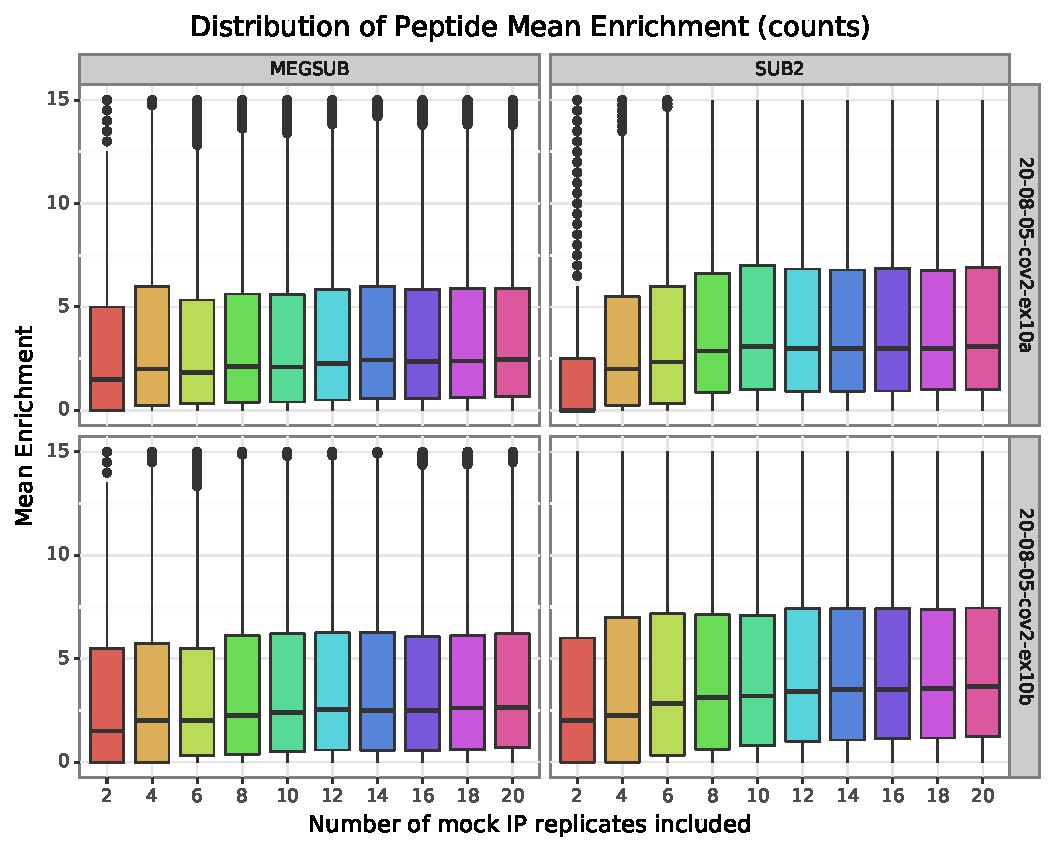
\includegraphics[width=65mm]{figures/42_mockip_abundance_variance/counts/mean_limit_y.pdf} &   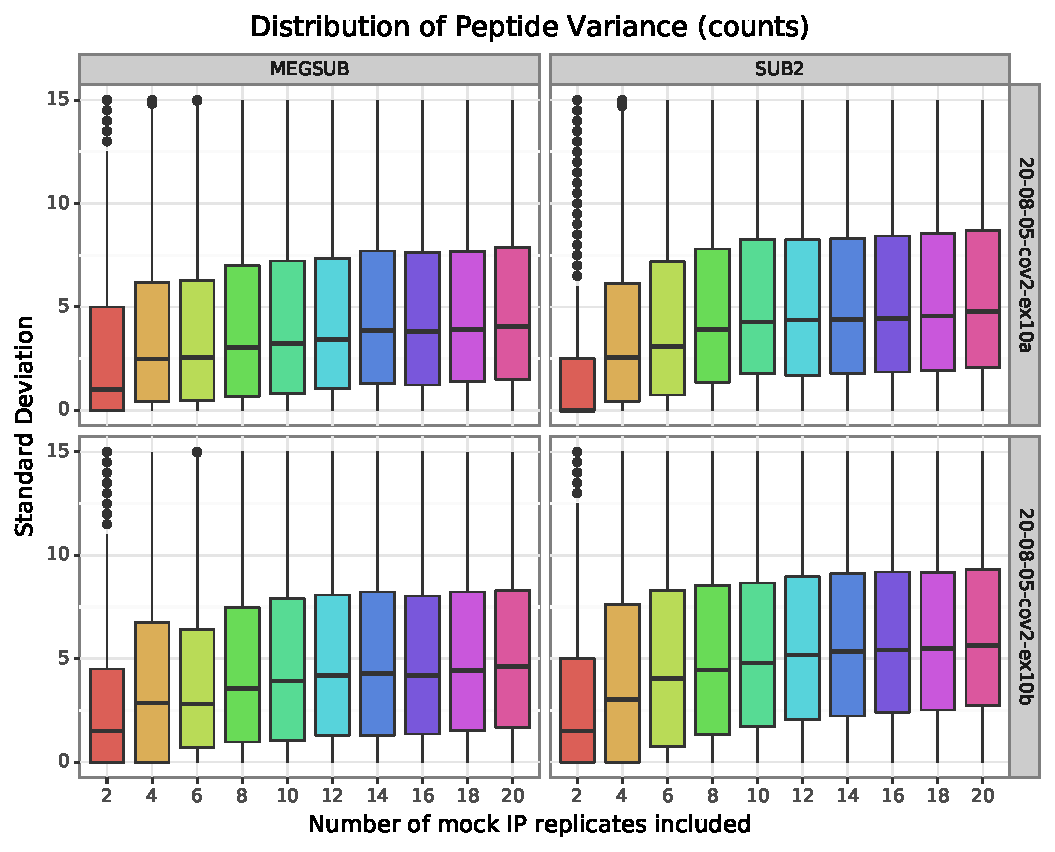
\includegraphics[width=65mm]{figures/42_mockip_abundance_variance/counts/std_limit_y.pdf} \\
(a) & (b) \\[6pt]
\multicolumn{2}{c}{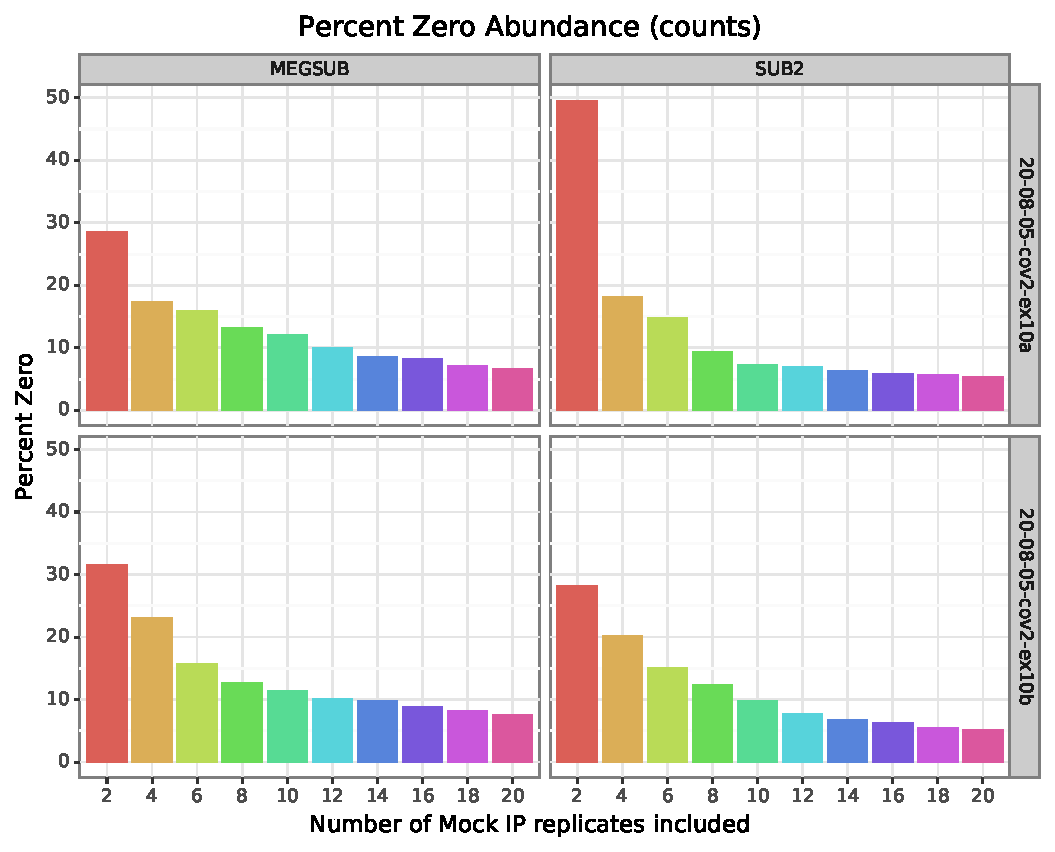
\includegraphics[width=85mm]{figures/42_mockip_abundance_variance/counts/per-zero.pdf} }\\
\multicolumn{2}{c}{(C)}
\end{tabular}
    \caption{A desciption of Negative control ``Mock-IP" sample using beads only with the library as described in \citet{Stoddard2020}. The pan-HCoV library includes just over 10,000 peptides. Each of the subfigures is a function of number of mock-IP's included when computing the each distribution. Each distribution to the right of another is a superset contianing all the previous Mock-IP's and all three sub-figures are the result of the same samples being chosen at each given Y. Each of the figures is facetted by both the library and experiment run to observe batch effects. (A) shows the distribution of mean enrichments across all peptides as a function of including more negative control samples. (B) shows the distribution of peptide variace as computed by each individual standard deviation, also as a function of adding more negative controls. (C) The number of peptides which have zero abundance (i.e their counts were zero) across all mock-IP's repoted as a percentage of all peptides in the library. The figure was generated independently and the data was derived from \citet{Stoddard2020}.} 
\label{fig:Mock-IP}
\end{figure}

\begin{figure}[h]
\centering
\includegraphics[width=0.85\textwidth]{figures/DMS-Cartoon.jpg}
    \caption{Deep mutational scanning. (A) Schematic of a deep mutational scanning experiment. Change in the abundance of variants is tracked by next-generation sequencing of DNA variants before and after selection for the function of the protein. The enrichment ratio (E) is a measure of the performance of each variant. (B) A sequence–function map of log2 enrichment ratios (E) for variants with a single amino acid change in a portion of the Pab1 protein. Blue, white, and red boxes represent variants that were depleted, neutral, or enriched, respectively, during the selection process; gray represents that no data passed quality filters; boxed with white dots represent the wild-type residue. - \citep{Starita2015}}
\label{fig:DMS-Cartoon}
\end{figure}

\begin{figure}[h]
\centering
\includegraphics[width=0.65\textwidth]{figures/Starr-Geno-Pheno.jpg}
    \caption{Sequence-to-Phenotype Maps of the SARS-CoV-2 RBD (A and B) Heatmaps illustrating how all single mutations affect RBD expression (A) and ACE2-binding affinity (B). Interactive versions of these heatmaps are at https://jbloomlab.github.io/SARS-CoV-2-RBD\_DMS and in Data S1. Squares are colored by mutational effect according to scale bars on the left, with red indicating deleterious mutations. The SARS-CoV-2 amino acid is indicated with an “x” and the SARS-CoV-1 amino acid, if different, is indicated with an “o”. Black boxes in top overlay indicate residues that contact ACE2 in the SARS-CoV-2 or SARS-CoV-1 crystal structures. The purple overlay represents the relative solvent accessibility (RSA) of a residue in the ACE2-bound SARS-CoV-2 crystal structure. See also Figure S3, Table S2, and Data S1. - \citep{Starr2020}}
\label{fig:Starr-Geno-Pheno}
\end{figure}
\end{document}
